\section{Compréhension et représentation de l'information incertaine}\label{representation}

\subsection{Une vision subjectiviste de la théorie bayésienne}

La fonction de co\^ut et le processus décisionnel permettent de proposer une \textcolor{black}{interprétation importante de la distribution {\it a priori}}. Elle peut \^etre comprise comme \textcolor{black}{pari} (personnel) fait sur l'éventualité d'un évènement, et notamment un gain conditionné par l'occurence du phénomène modélisé par $f(x|\theta)$. Cette interprétation \textcolor{black}{subjective}, proposée par de Finetti (1948), est certainement le point le plus critiqué de la démarche bayésienne, mais c'est aussi celui qui permet à l'application de cette théorie d'être ancrée dans le réel. \\

On peut en fait mieux appréhender cette interprétation subjectiviste en la reliant à l'histoire récente de l'axiomatique de la connaissance incertaine. 

\subsection{Théories de la connaissance incertaine}

Dans l'histoire des \textcolor{black}{théories de représentation mathématique de la connaissance incertaine}, il existe essentiellement deux grandes écoles de pensée :
\begin{enumerate}
\item des \textbf{théories de la représentation qui s'adaptent} aux moyens variés, pour un humain, d'exprimer son opinion personnelle sur le comportement d'une \textcolor{black}{variable d'ancrage} $X$ ou d'un paramètre perceptible $\theta$ (plus rare) ; 
\begin{itemize}
\item \emph{Exemples} : {théories extra-probabilistes : Dempster-Schafer, possibilités, logique floue ...} 
\end{itemize} 
\item des \textbf{théories qui visent à établir des \textcolor{black}{axiomes de rationalité}} à propos des décisions sous-tendant l'expression d'une opinion : un expert est per\c cu comme un \textcolor{black}{preneur de décision} selon ces axiomes.
\end{enumerate}

Une vision axiomatique de la représentation mathématisée de la connaissance incertaine, qui permet d'interpréter la théorie des probabilités comme une "bonne" fa\c con de représenter cette connaissance (ou plutôt cette information), a été construite par Cox et Jaynes. Elle s'incarne dans le théorème de Cox-Jaynes, dont les versions successives, au cours du temps, sont devenus les théorèmes fondamentaux de l'intelligence artificielle. Ce théorème permet de donner un cadre plus robuste à la vision subjectiviste du sens d'un modèle {\it a priori}. \\

\subsection{Une vision plus claire de la statistique bayésienne}

En définitive, il apparaît après ces premiers chapitres que la {statistique bayésienne} est à la fois :
\begin{itemize}
\item une théorie de la description d'un phénomène incertain, où ``incertitude" signifie ``mélange d'aléatoire (incertitude non-réductible) et d'épistémique (incertitude réductible) ;
\item une théorie de la décision, sous certains axiomes de rationalité.
\end{itemize}

Sachant un modèle $f(x|\theta)$, \textcolor{black}{le travail bayésien} consiste donc à:
\begin{enumerate}
\item déterminer le co\^ut associé aux décisions, $L(\theta,\delta)$ ;
\item éliciter ("construire") une loi {\it a priori} $\pi(\theta)$ ; 
\item réaliser l'inférence {\it a posteriori} et produire un ou plusieurs estimateurs, voire faire un choix de modèle. 
\end{enumerate}


Notons qu'il y a \textcolor{black}{redondance} entre les deux premières étapes : 
 présupposer l'existence d'une fonction de co\^ut implique qu'une certaine information {\it a priori} sur le problème considéré est disponible. \\
 
 La figure \ref{illust-bayes} illustre le positionnement classique de la vraisemblance statistique $f({\bf x_n}|\theta)$, vue comme une fonction de $\theta$, par rapport aux densit\'es $\pi(\theta)$ et $\pi(\theta|{\bf x_n})$ ; la mutualisation des sources d'information sur $\theta$ se traduit logiquement par une distribution {\it a posteriori} plus ``piqu\'ee" -- plus informative donc -- que la loi {\it a priori}\footnote{Except\'e dans les cas o\`u les deux sources d'information sont en d\'esaccord : voir \cite{Evans2006}.}. \\



\begin{figure}[h!]
\centering
\vspace{2cm}
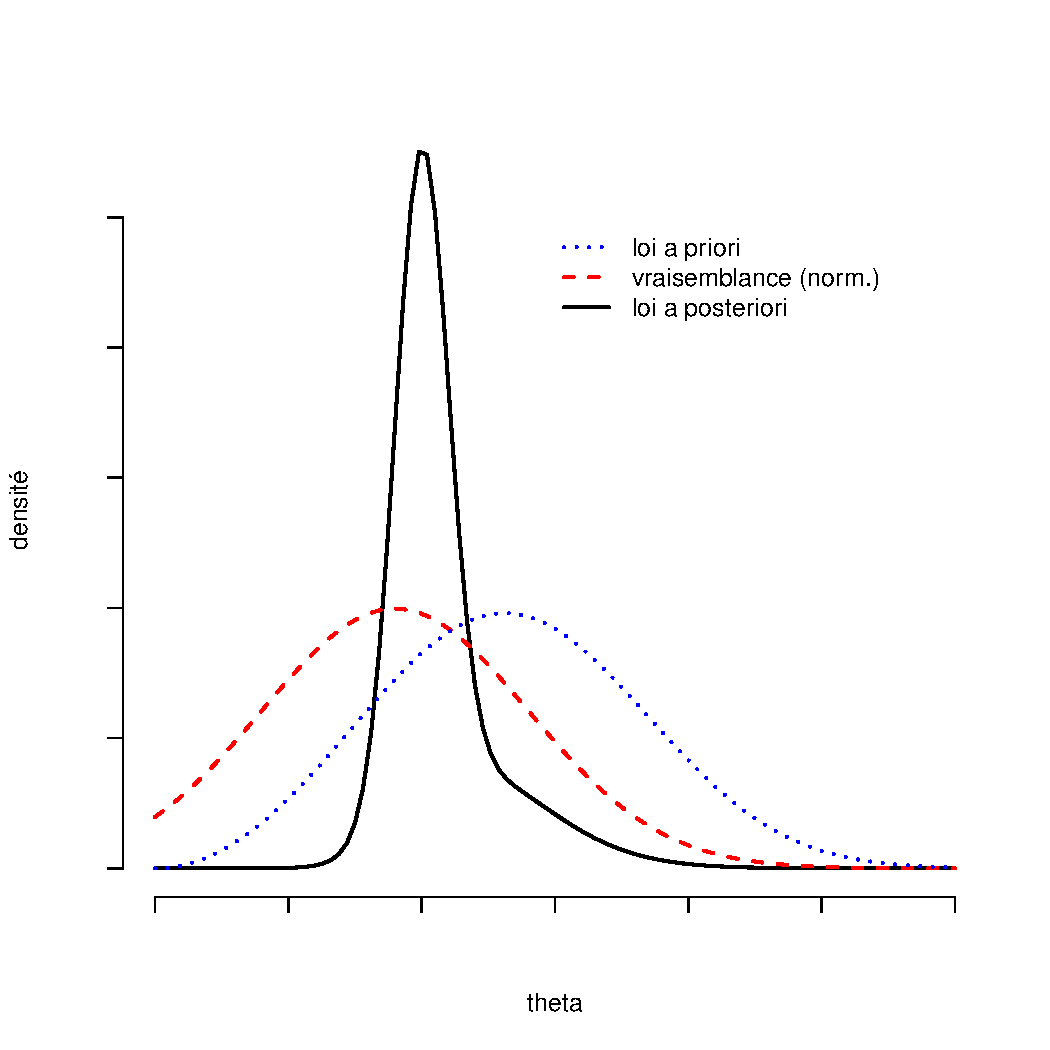
\includegraphics[scale=0.56,natwidth=380,natheight=380]{figures/ex-bayes-1.pdf}
\caption{Illustration par les densit\'es du renforcement de l'information sur $\theta$ \`a partir de la loi {\it a priori} et la vraisemblance des donn\'ees (vue comme fonction de $\theta$ et ici renormalis\'ee). }
\label{illust-bayes}
\end{figure} 




\paragraph*{\bf Nature de la loi {\it a priori}.}
 Qu'exprime la loi {\it a priori} $\pi(\theta)$ ? Un \'etat d'information initial sur les valeurs possibles de $\theta$, ind\'ependant des observations ${\bf x_n}$. Encod\'e sous forme probabiliste, cet \'etat d'information est donc susceptible de permettre l'ajout d'une connaissance r\'eelle et s\'erieuse du ph\'enom\`ene exprim\'ee autrement  qu'au travers d'observations pass\'ees : expertise, pr\'evisions de mod\`eles physiques, etc. Il faut noter que l'information {\it a priori} sur $\theta$ n'est jamais inexistante : en effet, $\theta$ est un choix de param\'etrisation du mod\`ele de statistiques extr\^emes choisi (type MAXB ou POT), et la structure de ce mod\`ele est connue. En d\'ecoulent des contraintes sur la structure de corr\'elation de $\pi(\theta)$ (cf. $\S$ \ref{elicitation}). Nous conseillons au lecteur int\'eress\'e par une pr\'esentation didactique des possibles interpr\'etations de $\pi(\theta)$ l'ouvrage \cite{Parent2007} et l'article \cite{Pasanisi2012}. 


\subsection{Validité des priors informatifs {\it via} la logique probabiliste de l'information incertaine}

Un prior informatif est la représentation probabiliste d'une information {\it a priori}, généralement sur $X$ (et non sur $\theta)$ {\it a piece of information  whose the value of truth is justified by considerations independent on experiment on focus} (Pegny 2012). Cette information peut avoir pour origine :
\begin{itemize}
\item des résultats d'essais autres que les données  (par exemple sur des maquettes) ;
\item des spécifications techniques d'exploitation ;
\item des bornes physiques ;
\item des extractions de corpus référencés ;
\item des connaissances exprimés par des experts humains. \\
\end{itemize}

Cette dernière information est souvent \emph{incomplète}, toujours \emph{incertaine},  à cause  de la non-existence d'un système permettant {\it a priori} de vérifier si l'expertise est complète ou non ; mais aussi à cause  de la non-existence d'un système suffisament précis pour spécifier que  $X=x_0$ exactement (sauf dans des cas rares et pathologiques). \\

Se pose alors la question de la pertinence de la théorie des probabilités pour représenter une information incertaine. Celle-ci offre de nombreux avantages pratiques, mais est-elle \emph{auditable} ? La subjectivité qui semble inhérente à ce choix peut être un élément de critique fort et limiter la confiance dans les approches bayésiennes informatives. \`A cela, on peut tout d'abord tirer parti de nombreux travaux épistémologiques. \\

\paragraph{Hypothèse 1 (Lakatos, 1974).} 
 L'information sur l'état de la nature est cachée et partiellement révélée par une \emph{théorie consensuelle} ({\it au sens de Popper  (1972) : par décision mutuelle des protagonistes}) définissant l'\emph{objectivité} {[{Gelman2015}]}.
Dans ce cadre,  la connaissance est un "filtrage" de l'information 
\item Ce filtrage est produit par l'intervention de symboles, ou signes, afin de la \emph{transmettre} ou de \emph{l'implémenter}.  \\



\paragraph{Hypothèse 2 (issu des neurosciences)  \cite{Sanders2011,Salinas2011,Pouget2013,Gold2013,Dehaene2014,Chan2016}.}  Face à des situations où de l'information incertaine est mobilisée, le raisonnement humain produit des inférences probabilistes. Les difficultés apparaissent au moment de l'explicitation de cette information par  \emph{langage interprétatif} $\Rightarrow$ \emph{expertise utilisable}. \\

Sous ces hypothèses, nous ne savons pas comment définir formellement la  ``déconvolution" retransformant la connaissance incertaine en information incertaine. Mais nous pouvons avoir des idées sur l'impact de l'ajout d'une connaissance incertaine mais utile sur la résolution du problème de détermination de  $X$. Cet ajout se manifeste par un accroissement de l'information sur $X$ -- c'est-à-dire une \emph{inférence} (mise à jour): 
\begin{description}
\item[(a)] cette inférence doit s'appuyer sur un principe de raisonnement ;
\item[(b)] ce principe de raisonnement s'établit lui-même sur une  \emph{logique}, c'est-à-dire un ensemble de  {\bf règles formelles}. \\ 
\end{description}

Quelles propriétés souhaitons-nous pour cette logique ? Qu'elle permette de trier des assertions {\it atomiques} du type $X=x_0$ at chaque ajout d'information  ({\it logique exclusive}). Ainsi,  une situation initiale (\emph{prémisse}) doit être moins informatique qu'une conclusion (\emph{mise à jour}). De plus, cette logique doit permettre de de représenter une information {\it incertaine}  : on doit pouvoir trier plus d'assertions  que celles qui sont simplement vraies ou fausses  ({\it logique non-booléenne}). Construire une telle logique de l'information incertaine nécessite de définir les concepts suivants. \\

\begin{definition}{\bf \'Etat d'information.}
Soit $S_X$ un ensemble de propositions (assertions) atomiques du type $X=x_i$. L'ensemble $B_X$ de toutes les  {\it propositions composites} générées par 
\begin{eqnarray*}
\neg X=x_i, &  X=x_i \land X=x_j,  \\
 \ X=x_i \lor X=x_j, & X=x_i \Rightarrow X=x_j \\
 \text{and} & X=x_i \Leftrightarrow X=x_j
\end{eqnarray*} 
est appelé \emph{état d'information}, avec $\mbox{Dom}(B_X)=$ fermeture logique de $S_X$.
\end{definition}

L'état d'information $B_X$ résume l'information existante sur un ensemble de propositions portant sur $X$. Si la logique souhaitée précédemment existe, elle devrait guider la fa\c con dont  $B_X$ évolue : il croît selon une certaine métrique quand l'information sur $X$ croît. Pour mesurer cette croissance de l'information, il faut introduire le concept de plausibilité, qui lui-même permet le calcul propositionnel. \\


\begin{definition}{\bf Plausibilité.}
Considérons une proposition $A$ on $X$. Sachant $B_X$, la \emph{plausibilité} $[A|B_X]$ est un nombre réel, supérieurement borné par un nombre (fini ou infini) $T$.  
\end{definition}

Supposer que la plausibilité existe est un axiome dit de  \emph{non-ambigu\"ité} est particulièrement important\footnote{les différences entre logique probabiliste et logique non probabiliste (ou {\it extra-probabiliste}) sont issues de l'accord ou du désaccord avec cette hypothèse. Jaynes (1954)  justifie toutefois la validité de cette hypothèse sur des bases pragmatiques.}. Il produit  une hypothèse de {\it comparabilité universelle}\footnote{Cette hypothèse est notamment motivée lorsque nous parlons de quantités $X$ possédant une \emph{signification physique et prenant une unique valeur à chaque instant} (étant donnée, possiblement, une précision de mesure finie).}, qui a pour conséquence qu'une information additionnelle (pas forcément une connaissance)  peut seulement faire croître ou décroître la plausibilité d'une proposition. \\

\begin{definition}{\bf Consistance.}
$B_X$ est consistant s'il n'existe aucune proposition  $A$ pour qui  $[A|B_X]=T$ et $\neg[A|B_X]=T$.  
\end{definition}


\begin{definition}{\bf Calcul propositionnel.}
Le calcul propositionnel est un ensemble de règles  permettant à tout domaine de problème de formuler des propositions utiles. Il s'exprime ainsi :
\begin{eqnarray*}
\left.
\begin{array}{ll}
{\it (i)} & \text{Si $A=A'$ alors $[A|B_X] \Leftrightarrow [A'|B_X]$} \\
{\it (ii)} & \text{$[A|B_X,C_X,D_X]=[A|(B_X \land C_X),D_X]$} \\
{\it (iii)} & \text{Si $B_X$ est consistant et $\neg[A|B_X]<T$, alors $A\cup B_X$ est consistant} \\
\end{array}
\right. & %\begin{array}{l} \text{\tiny applicable to any problem domain for} \\
%\text{\tiny which we can formulate useful propositions}
%\end{array}
\end{eqnarray*}
\begin{itemize}
\item  {\bf Cohérence}: il existe une fonction non croissante  $S_0$ telle que, pour tout $x$ et tout $B_X$ consistant
\begin{eqnarray*}
\neg[A|B_X]=S_0([A|B_X])
\end{eqnarray*}
\item {\bf Densité} : l'ensemble $[S_0(T),T]$ admet un sous-ensemble non vide, dense et consistant.
\end{itemize}

\end{definition}

Ce calcul propositionnel, qui repose sur l'axiome de non-ambigu\"ité,  formalise donc des règles simples permettant de décrire les propriétés d'une logique de l'incertain. Celle-ci peut se vulgariser de la fa\c con suivante : 
\begin{enumerate}
\item \emph{Règle de reproductibilité} : deux assertions équivalentes sur $X$ ont la même plausibilité.
\item \emph{Règle de non-contradiction} : s'il existe plusieurs approches aboutissant aux même conclusions sur $X$, celles-ci ont la même plausibilité. 
\item \emph{Règle de consistence} : la logique ne peut formuler une conclusion contredite par les règles élémentaires de déduction (ex : transitivité). 
\item \emph{Règle d'integrité} : la logique ne peut exclure une partie de l'information sur $X$ pour parvenir à une conclusion sur $X$. 
\item \emph{Règle de monotonie} : la plausibilité d'une union non exclusive de deux assertions est au moins égale à la plus grande des plausibilités de chacune des assertions prises séparément. 
\item \emph{Règle de produit}: la plausibilité de l'intersection  de deux assertions est au plus égale à la plus petite des plausibilités de chacune des assertions prises séparément.  \\
\end{enumerate}

On arrive dès lors à la question suivante : d'un point de vue pratique, cette logique est-elle équivalente à une théorie mathématique connue de représentation de l'information ? Le théorème suivant, absolument fondamental pour justifier l'usage de la théorie des probabilités pour représenter un réel incertain, est initialement dû à Cox (1946) et Jaynes (1954). Il a été étendu plus rigoureusement par Paris (1994), Van Horn (2003), Dupré and Tipler (2009) (entre autres) et finalisé par Terenin and Draper (2015). Il indique que sous les axiomes précédents, une plausibilité se comporte exactement comme une probabilité. \\

\begin{theorem}{\bf Cox-Jaynes}
Sous les axiomes précédents, il existe une fonction $\Pp$, croissante et continue, telle que pour  toute proposition $A,C$ et tout ensemble $B_X$ consistant,
\begin{description}
\item[(i)] $\Pp([A|B_X])=0$ si et seulement si $A$ est fausse étant donnée l'information sur $X$
\item[(ii)] $\Pp([A|B_X])=1$ si et seulement si $A$ est vraie étant donnée l'information sur $X$  
\item[(iii)] $0\leq \Pp([A|B_X]) \leq 1$ 
\item[(iv)] $\Pp([A \land C|B_X])=\Pp([A |B_X])\Pp([C |A,B_X])$
\item[(v)] $\Pp(\neg [A|B_X]) = 1 - \Pp([A|B_X])$
\end{description} 
On en conclut que tout système de raisonnement plausible, sous les hypothèses précédentes, est isomorphe à la théorie des probabilités. 
\end{theorem}

Ce théorème est donc particulièrement fondamental en IA. Il est particulièrement résistant à la variation de certains axiomes. Ainsi, Goertzel (2013) a prouvé que si la règle de consistance était affaiblie, alors les plausibilités se comportent approximativement comme des probabilités. On en conclut La théorie des probabilités est pertinente pour représenter les incertitudes sur un sujet exploré par un systèmes cognitif implicite (humain ou artificiel) qui pourrait ne pas être complément consistant. \\

